\documentclass[11pt]{article}
\usepackage[final]{acl}
\usepackage{times}
\usepackage{latexsym}
\usepackage[T1]{fontenc}
\usepackage[utf8]{inputenc}
\usepackage{microtype}
\usepackage{graphicx}
\usepackage{booktabs}
\usepackage{xcolor}
\usepackage{multirow}
\graphicspath{{../results/figures/}}

% generated by report/make_numbers.py - do not edit by hand
\newcommand{\AGbi}{92.34}
\newcommand{\AGbiSD}{0.10}
\newcommand{\AGbiMin}{92.22}
\newcommand{\AGbiMax}{92.45}
\newcommand{\AGbiT}{4.8}
\newcommand{\AGbiFone}{92.3}
\newcommand{\AGuni}{91.43}
\newcommand{\AGuniSD}{0.05}
\newcommand{\AGuniMin}{91.36}
\newcommand{\AGuniMax}{91.47}
\newcommand{\AGuniT}{3.2}
\newcommand{\AGuniFone}{91.4}
\newcommand{\NGpaper}{16.41}
\newcommand{\NGpaperSD}{0.17}
\newcommand{\NGpaperMin}{16.21}
\newcommand{\NGpaperMax}{16.67}
\newcommand{\NGpaperT}{2.3}
\newcommand{\NGpaperFone}{9.6}
\newcommand{\NGep}{62.17}
\newcommand{\NGepSD}{0.18}
\newcommand{\NGepMin}{61.96}
\newcommand{\NGepMax}{62.37}
\newcommand{\NGepT}{7.0}
\newcommand{\NGepFone}{61.1}
\newcommand{\NGhs}{56.97}
\newcommand{\NGhsSD}{0.42}
\newcommand{\NGhsMin}{56.53}
\newcommand{\NGhsMax}{57.67}
\newcommand{\NGhsT}{6.7}
\newcommand{\NGhsFone}{56.3}
\newcommand{\RSSin}{37.22}
\newcommand{\RSSinSD}{7.72}
\newcommand{\RSSinMin}{28.71}
\newcommand{\RSSinMax}{44.55}
\newcommand{\RSSinT}{0.5}
\newcommand{\RSSinFone}{28.1}
\newcommand{\AGtf}{92.58}
\newcommand{\AGtfT}{71.9}
\newcommand{\AGtfFone}{92.6}
\newcommand{\NGtf}{76.53}
\newcommand{\NGtfT}{54.7}
\newcommand{\NGtfFone}{75.5}
\newcommand{\RSStf}{72.28}
\newcommand{\RSStfT}{0.1}
\newcommand{\RSStfFone}{71.2}
\newcommand{\AGgap}{-0.16}
\newcommand{\AGtfGap}{0.24}
\newcommand{\AGperEpoch}{1.0}
\newcommand{\AGuniGap}{-0.07}
\newcommand{\AGbigramGain}{0.9}
\newcommand{\AGspeedup}{15}
\newcommand{\NGspeedup}{8}
\newcommand{\AGrecWorld}{92.2}
\newcommand{\AGrecSports}{98.0}
\newcommand{\AGrecBusiness}{89.3}
\newcommand{\AGrecSciTech}{89.8}
\newcommand{\NGbest}{66.50}
\newcommand{\NGbestSD}{0.39}
\newcommand{\NGbestEp}{100}
\newcommand{\NGbestLr}{0.25}
\newcommand{\NGbestT}{20.4}
\newcommand{\NGbestGap}{10.0}
\newcommand{\DimAx}{62.35}
\newcommand{\DimAxT}{6.6}
\newcommand{\DimAl}{62.75}
\newcommand{\DimAlT}{10.7}
\newcommand{\DimAc}{62.25}
\newcommand{\DimAcT}{16.0}
\newcommand{\DimBx}{64.80}
\newcommand{\DimBxT}{3.0}
\newcommand{\DimBl}{65.31}
\newcommand{\DimBlT}{5.5}
\newcommand{\DimBc}{64.56}
\newcommand{\DimBcT}{8.3}
\newcommand{\DimMaxChange}{0.5}
\newcommand{\XF}{74.41}
\newcommand{\XFSD}{0.50}
\newcommand{\XFn}{508}
\newcommand{\XFdrop}{17.9}
\newcommand{\XFrecWorld}{81.7}
\newcommand{\XFrecSports}{82.1}
\newcommand{\XFrecBusiness}{59.1}
\newcommand{\XFrecSciTech}{72.0}
\newcommand{\JudgeN}{127}
\newcommand{\JudgeModel}{55}
\newcommand{\JudgeModelPct}{43}
\newcommand{\JudgeAmb}{37}
\newcommand{\JudgeAmbPct}{29}
\newcommand{\JudgeNoise}{35}
\newcommand{\JudgeNoisePct}{28}
\newcommand{\XFseedZero}{75.00}
\newcommand{\XFnoNoise}{80.5}
\newcommand{\XFlenient}{88.4}
\newcommand{\HumanN}{30}
\newcommand{\HumanAgree}{47}
\newcommand{\HumanKappa}{0.20}
\newcommand{\HumanBinary}{63}


\title{Does a Bag of Tricks Still Work Twenty Years Later?\\
Replicating fastText on AG News, 20 Newsgroups and 2026 News Headlines}

\author{Subbareddy Pullalacheruvu \\
  48641626 \\
  Macquarie University \\
  \texttt{subbareddy.pullalacheruvu@students.mq.edu.au}}

\begin{document}
\maketitle

\begin{abstract}
I replicate the AG News result of \citet{joulin-etal-2017-bag}, who introduced fastText, a
linear text classifier that the authors report is about as accurate as much slower deep
models. With the authors' own code and hyperparameters, five seeds give \AGbi\%~$\pm$~\AGbiSD{}
against the paper's 92.5\% (with bigrams), and \AGuni\% against 91.5\% (unigrams only). The
result replicates. I then test the paper's speed-versus-accuracy claim on data it never
used. On 20~Newsgroups (20 classes, long posts, small training set) the paper's
configuration reaches only \NGpaper\%. Even after tuning, fastText stays \NGbestGap{}
points behind a TF-IDF logistic regression baseline, although it is still much faster. On a
new dataset of 548 news headlines I collected from RSS feeds in October 2026, a model trained
on 2004-era AG News falls from \AGbi\% to \XF\%. An LLM-as-judge analysis of these errors
and a human check of the judge suggest that part of this drop comes from label noise and
ambiguous headlines rather than model failure, although the judge and I agreed only
slightly on which errors were which. The code, the new dataset and all results are public.\footnote{%
\url{https://github.com/subbareddypullalacheruvu/fasttext-replication}}
\end{abstract}

% ===================================================================
\section{Introduction}

Open code and data are meant to make results checkable, but a result is only useful if
it holds when someone else runs the code and when the data changes. This project asks
both questions of one widely used paper. Phase~1 reruns the authors' code on their own
AG News data. Phase~2 runs the same pipeline on an existing dataset the paper did not
test (20~Newsgroups) and on a dataset I built myself: news headlines from 2026, in the
same four classes and format as AG News, collected about twenty years after it. The
question running through both phases is whether fastText's ``nearly as accurate, much
faster'' trade-off is a property of the method or a property of AG News.

% ===================================================================
\section{The Paper and Why It Was Chosen}

\paragraph{The paper.} \citet{joulin-etal-2017-bag} propose a deliberately simple text
classifier. Each document is treated as an unordered bag of words and word bigrams. Each
word or bigram has a small learned embedding, and bigrams are hashed into a fixed number of
buckets so memory stays bounded. The document vector is the average of these embeddings,
and a single linear layer with a softmax (or a hierarchical softmax when there are many
classes) predicts the label. There are no convolutions, recurrence or attention. The paper
claims that on eight standard sentiment and topic datasets this model is ``often on par''
with deep models while training in seconds on a CPU.\footnote{%
\url{https://aclanthology.org/E17-2068/}}

\paragraph{Evaluation framework.} The paper reports test \emph{accuracy}, the fraction of
test documents given the correct label, on the eight datasets of \citet{zhang2015character},
alongside training time. All eight are single-label, so accuracy is well defined, and
fastText's precision@1 and recall@1 equal accuracy. On AG News the paper reports
91.5\% (unigrams, 10 hidden units, 5 epochs) and 92.5\% with bigrams. For comparison, the
character-level CNN of \citet{zhang2015character} reaches 87.2\% and their word n-gram TF-IDF
model 92.4\%.

\paragraph{Justification.} The paper appeared at EACL 2017, which is ranked~A by ICORE
\citep{icore2026} and is one of the four main conferences of the Association for
Computational Linguistics, alongside ACL, NAACL and EMNLP.
It has about 5,300 citations on Google Scholar (2026), and the official
repository\footnote{\url{https://github.com/facebookresearch/fastText}} has about 26.5k
stars. The code and data are freely available, and the experiments run on a laptop CPU,
so a full replication is feasible. One risk was that the repository was archived in March
2024. Its last release (v0.9.2) still installs as \texttt{fasttext-wheel} on Python~3.11.

% ===================================================================
\section{The Original Datasets}

\paragraph{All datasets in the paper.} The paper evaluates on the eight text classification
datasets of \citet{zhang2015character}, listed in Table~\ref{tab:datasets}, and separately on
tag prediction with YFCC100M, a set of almost 100 million Flickr images. For tag prediction
it uses only the titles and captions: 91.2M training examples, 543k test examples and
312k unique tags. I replicate AG News, the smallest of the classification datasets and the
one whose news domain my new data continues. Replicating all eight was outside the time I
had: the two Amazon sets alone hold 3.0M and 3.6M training reviews, and YFCC100M runs to 1.5 billion
tokens.

\begin{table}[t]
\centering\small
\begin{tabular}{@{}lrrrc@{}}
\toprule
Dataset & Classes & Train & Test & Paper \\
\midrule
AG News & 4 & 120k & 7.6k & 92.5 \\
Sogou News & 5 & 450k & 60k & 96.8 \\
DBpedia & 14 & 560k & 70k & 98.6 \\
Yelp Polarity & 2 & 560k & 38k & 95.7 \\
Yelp Full & 5 & 650k & 50k & 63.9 \\
Yahoo! Answers & 10 & 1.4M & 60k & 72.3 \\
Amazon Full & 5 & 3.0M & 650k & 60.2 \\
Amazon Polarity & 2 & 3.6M & 400k & 94.6 \\
\bottomrule
\end{tabular}
\caption{The eight classification datasets used by \citet{joulin-etal-2017-bag}, from
\citet{zhang2015character}. ``Paper'' is fastText's test accuracy (\%) with bigrams,
$h=10$.}
\label{tab:datasets}
\end{table}

\paragraph{AG News.} AG News \citep{zhang2015character} was built from a news corpus gathered by the
ComeToMyHead academic search engine from more than 2,000 sources, mostly in 2004--2005. It has
four balanced classes (World, Sports, Business, Sci/Tech), with 30,000 training and 1,900 test
items per class (120,000 / 7,600 in total). Each item is a headline and a short description,
usually the first sentence of the article, about 45 tokens on average. The data is
distributed as two CSV files with columns \emph{class index, title, description}
(Figure~\ref{fig:agnews}).\footnote{\url{https://github.com/mhjabreel/CharCnn_Keras/tree/master/data/ag_news_csv}}
I checked the copy I used rather than assuming it was correct. The row counts and per-class
counts are exact, there are no empty fields or duplicate rows, and the first record matches
the canonical one quoted in other sources.

\begin{figure}[t]
\footnotesize
\begin{verbatim}
"3","Wall St. Bears Claw Back Into
 the Black (Reuters)","Reuters -
 Short-sellers, Wall Street's
 dwindling\band of ultra-cynics,
 are seeing green again."
\end{verbatim}
\vspace{-4pt}
After the authors' \texttt{normalize\_text}:
\begin{verbatim}
__label__3 , wall st . bears claw
 back into the black ( reuters ) ,
 reuters - short-sellers , ...
\end{verbatim}
\vspace{-6pt}
\caption{An AG News training item as distributed (top) and in fastText input format
(bottom). Class 3 is Business.}
\label{fig:agnews}
\end{figure}

% ===================================================================
\section{Replication of the Original Work}

\paragraph{Environment and procedure.} I used the authors' release v0.9.2 through the
\texttt{fasttext-wheel} Python package, with the hyperparameters from the authors'
\texttt{classification-results.sh}: \texttt{dim=10}, \texttt{lr=0.25},
\texttt{wordNgrams=2}, \texttt{minCount=1}, \texttt{bucket=10M}, \texttt{epoch=5}, softmax
loss. The authors preprocess with a \texttt{sed}/\texttt{tr} pipeline
(\texttt{normalize\_text}). I ported it to Python and checked it line by line against the
shell output, so the model sees the same tokens. The first setup on Windows~11 failed twice.
\texttt{fasttext-wheel} needs the Microsoft C++ build tools, and its binding breaks with
NumPy~2, so \texttt{numpy<2} is pinned. Training is stochastic (Hogwild SGD with random
initialisation), so I ran five seeds (0--4) with two threads and report mean $\pm$ standard
deviation. As a comparison model that the paper does not include, I trained a TF-IDF
(word 1--2 grams) logistic regression on the same input.

My first runs (Windows~11, 9 October 2026) gave 92.25--92.37\% on AG News. The results file
from those runs is archived in the repository. The numbers in this report were regenerated in a single batch
with the same package versions (Python~3.11, \texttt{fasttext-wheel}~0.9.2,
NumPy~1.26) on a Linux machine, so that every result comes from the same run of
\texttt{results.json}. The two environments agree closely: AG News results differ by at most
0.08 points, and 20~Newsgroups results by at most 0.4 points.

\begin{table}[t]
\centering\small
\begin{tabular}{lccr}
\toprule
Model & Paper & Mine (5 seeds) & Train \\
\midrule
fastText, unigrams & 91.5 & \AGuni{} $\pm$ \AGuniSD & \AGuniT\,s \\
fastText, + bigrams & 92.5 & \AGbi{} $\pm$ \AGbiSD & \AGbiT\,s \\
TF-IDF + LogReg & -- & \AGtf & \AGtfT\,s \\
\bottomrule
\end{tabular}
\caption{AG News test accuracy (\%). ``Paper'' is Table~1 of
\citet{joulin-etal-2017-bag}. Training time is wall-clock seconds on the same CPU machine (2 threads) for every model.}
\label{tab:repl}
\end{table}

\paragraph{Results and closeness.} Table~\ref{tab:repl} shows the result. The bigram model
reaches \AGbi\%, a gap of \AGgap{} points from the paper. The five seeds span
\AGbiMin--\AGbiMax\%, so the remaining gap is about the size of seed-to-seed variation. The unigram model (gap \AGuniGap) and the gain
from adding bigrams (+\AGbigramGain{} points, against +1.0 in the paper) also replicate. The
small remaining difference is most likely due to random initialisation and thread
scheduling. The paper reports a single run and does not give its seed or thread count. The
paper's speed claim is made against deep models. Its Table~2 reports one training epoch on AG
News taking 1\,h for the small char-CNN and 24\,min for the smallest VDCNN, against 1\,s for
fastText. I did not rerun the deep models, but my fastText time agrees with the paper's:
\AGbiT\,s for five epochs, about \AGperEpoch\,s per epoch. As an extra baseline the paper does not
include, the TF-IDF model is only \AGtfGap{} points more accurate (\AGtf\%) but takes about
\AGspeedup{} times longer to train. So fastText is fast compared with linear models too, not
only compared with deep ones.

\paragraph{Where it works and where it fails.} Recall is highest for Sports (\AGrecSports\%)
and lowest for Business (\AGrecBusiness\%) and Sci/Tech (\AGrecSciTech\%). Most errors are
Business~$\leftrightarrow$~Sci/Tech confusions about technology companies, where the
headline mentions a technology firm but the story is about money. Some ``errors'' are
problems in AG News itself. For example, a Tata Consultancy share listing is labelled
\emph{World}, and a Nortel revenue warning is labelled \emph{Sci/Tech}. The model's
predictions (Business) are arguably better than the gold labels in both cases. Many
remaining errors are deals between technology firms, where either label can be defended.
\emph{``PeopleSoft, IBM strike middleware alliance''} is gold Sci/Tech but predicted
Business, and \emph{``I.B.M. sought a China partnership, not just a sale''} is gold Business
but predicted Sci/Tech. The second also shows a tokenizer side effect that matters later: the
authors' \texttt{normalize\_text} splits ``I.B.M.'' into \emph{i~.~b~.~m~.}, so the
abbreviation never appears as one word.

% ===================================================================
\section{Construction of New Data}

\subsection{20 Newsgroups (existing dataset)}
20~Newsgroups \citep{lang1995newsweeder} is a collection of Usenet posts from 20 discussion
groups. I used the standard ``bydate'' training portion (11,314 posts) as a single JSON
file.\footnote{\url{https://github.com/selva86/datasets}} It differs from AG News in three
ways. It has 20 classes instead of 4. Its posts average 262 tokens instead of 45. And it has
13 times less training data. Raw posts contain \texttt{Newsgroups:} headers, email
addresses and signatures that give away the label, so I removed headers, signatures and
quoted replies with scikit-learn's standard functions. Posts with fewer than three
remaining words were dropped. That leaves 10,959 posts, split 80/20 with stratification
(seed 42) into 8,769 training and 2,190 test posts.

\subsection{UCI News Aggregator (descoped)}
My proposal also planned the UCI News Aggregator dataset \citep{gasparetti2017uci}. I wrote
its preprocessing, but did not run it, for two reasons. Only two of its four classes
(business, sci/tech) overlap with AG News, so it cannot test transfer from AG News the way
the 2026 data can. And with the time left, the LLM-as-judge analysis was a better use of
it. The code path (\texttt{preprocess.py uci}) is in the repository.

\subsection{2026 RSS headlines (new dataset)}
The point of this dataset is a question AG News cannot answer by itself. AG News describes
news language of 2004. Does a model trained on it still work on news written in 2026,
where Sci/Tech is dominated by AI and data centres?

\paragraph{Collection.} \texttt{collect\_rss.py} reads 15 public RSS section feeds from
the BBC, The Guardian, The New York Times and ESPN. Each item gets the AG News label of the
section it was published in. For example, BBC \emph{world} maps to World, Guardian
\emph{technology} to Sci/Tech, and NYT \emph{business} to Business. The NYT sports feed
returned nothing, so ESPN replaced it. For every item I keep the source, section, link,
publication time and collection time. Two collection runs on 9~October 2026 produced 548
unique items.

\paragraph{Processing.} I strip HTML and feed boilerplate, and cut the description to its
first sentence to match AG News. This did not always work. The Guardian's summaries often
have no sentence break, and the feed truncates them at a fixed length, so 93 of the 508
usable leads (84 of them from the Guardian) end mid-word or mid-sentence. Another 20
Guardian leads still contain sign-up text (``Get our breaking news email\ldots''), which my
boilerplate filter missed. Four items are promotions or carry no real headline (``Here's
the latest.'', ``Find out more here'', ``Football Daily'', ``The Bottom Line''). The
spot-check caught one of these, but I did not remove them. They are under 1\% of the data
and are still included in the frozen version, so the reported results contain them. Duplicates are removed by link and by normalised headline.
Then the same \texttt{normalize\_text} as for AG News is applied. Forty stories appeared in
two different sections, for example both World and Business. Their label is ambiguous by
construction, so I flag and exclude them. That leaves \textbf{508 usable items}: World 127,
Sports 135, Business 106, Sci/Tech 140, averaging 37 words (Figure~\ref{fig:rss}).

\begin{figure}[t]
\small
\begin{tabular}{@{}p{0.94\columnwidth}@{}}
\toprule
\textbf{World} (BBC \emph{world}) \textbullet{} Suspect linked to Monaco bomb attack on
millionaire breaks silence to BBC \textbar{} Vitalii Zhykovych gives his own account of
the attempted assassination\ldots\\
\midrule
\textbf{Sports} (BBC \emph{sport}) \textbullet{} Toone comes into England squad as Bronze
withdraws \textbar{} Manchester United midfielder Ella Toone receives a late England
call-up\ldots\\
\midrule
\textbf{Sci/Tech} (Guardian \emph{technology}) \textbullet{} How Zach Cregger's Resident
Evil stands out from all other game adaptations \textbar{} There's no Leon, Claire or Ada
Wong\ldots\\
\bottomrule
\end{tabular}
\caption{Items from the 2026 RSS dataset: label (feed), headline \textbar{} lead sentence.
The third shows a weakness of section labels: a film review filed under technology.}
\label{fig:rss}
\end{figure}

\paragraph{Annotation and agreement.} There was no budget for crowdsourcing, so the labels
come from the outlets' sections and are checked by hand. I wrote a one-page labelling
guideline that defines each class, gives exclusions and adds a tie-break rule (``what the
story is \emph{mainly} about''). I then checked a random sample of 50 usable items against
it. 45 of the 50 labels were correct (\textbf{90\% agreement}), above the 85\% threshold I had
set in advance for keeping the feed-to-label mapping. The five disagreements were two
technology-policy stories filed as Sci/Tech that the guideline puts in World (for example,
Finland halting two Google data centres), one arts story that fits no class, one feed item
with no real headline, and one environment report. This is single-annotator agreement with
the automatic labels, not inter-annotator agreement, because no second annotator was
available.

\paragraph{Known limitations.} The dataset is small and comes from a single day. It is
Anglophone (UK and US outlets). Source and class are confounded: ESPN contributes only Sports
and NYT no Sports. Guardian leads are often truncated or contain boilerplate, as described
above. I froze the dataset at
this version for the report rather than keep collecting.

% ===================================================================
\section{Results on New Data}

\begin{table}[t]
\centering\small
\begin{tabular}{@{}llcr@{}}
\toprule
Data & Model & Acc. (\%) & Train \\
\midrule
\multirow{2}{*}{AG News} & fastText (paper cfg) & \AGbi & \AGbiT\,s \\
 & TF-IDF + LogReg & \AGtf & \AGtfT\,s \\
\midrule
\multirow{5}{*}{20NG} & fastText (paper cfg) & \NGpaper{} $\pm$ \NGpaperSD & \NGpaperT\,s \\
 & fastText, 25 ep. & \NGep{} $\pm$ \NGepSD & \NGepT\,s \\
 & \quad + hier.\ softmax & \NGhs{} $\pm$ \NGhsSD & \NGhsT\,s \\
 & fastText, best (\NGbestEp{} ep.) & \NGbest{} $\pm$ \NGbestSD & \NGbestT\,s \\
 & TF-IDF + LogReg & \NGtf & \NGtfT\,s \\
\midrule
2026 & AG News $\rightarrow$ 2026 & \XF{} $\pm$ \XFSD & -- \\
\bottomrule
\end{tabular}
\caption{Results on new data, five seeds for fastText. ``Paper cfg'' is the paper's
AG News configuration unchanged. AG News $\rightarrow$ 2026 is trained on all of AG News and tested on the
\XFn{} usable 2026 items.}
\label{tab:new}
\end{table}

\subsection{20 Newsgroups: the configuration does not transfer}
With the paper's AG News settings, fastText reaches only \NGpaper\% on 20~Newsgroups
(Table~\ref{tab:new}). It has not failed in principle. It is under-trained: 5 epochs over
8,769 documents is about 14 times fewer document updates than on AG News, and the learning
rate decays to zero over those few updates. An epoch and learning-rate
sweep (Figure~\ref{fig:sweep}) shows accuracy climbing to \NGbest\% at \NGbestEp{} epochs,
lr\,=\,\NGbestLr. This best setting was chosen on the test set (there is no separate
development split), so \NGbest\% is optimistic. The gap to the untuned TF-IDF baseline is
large enough that this does not change the conclusion. A higher learning rate (1.0) gets most of the way much sooner: 65.1\% after
only 10 epochs and 2.8\,s. Either way, accuracy then plateaus \NGbestGap{} points below TF-IDF logistic regression
(\NGtf\%). The \emph{speed} half of the claim survives: fastText still trains several times
faster (\NGepT\,s against \NGtfT\,s at 25 epochs). The \emph{accuracy} half does not. I tested
one obvious explanation, that the 10-dimensional hidden layer is too small for 20 classes. It
is not the cause. With dim\,=\,50 or 100, accuracy changes by at most \DimMaxChange{} points
(25 epochs: \DimAx, \DimAl{} and \DimAc\%; lr\,=\,1.0 and 10 epochs: \DimBx, \DimBl{} and
\DimBc\%, for dim 10, 50 and 100), while training takes 2.4--2.8 times longer. These are
separate runs from Table~\ref{tab:new} and the epoch sweep. Multi-threaded fastText is not
bit-reproducible, so repeated runs of the same setting differ by a few tenths of a point. The more
likely causes are that averaging over long documents dilutes the few informative words, and
that the training set is small. Hierarchical softmax costs accuracy
(\NGhs\% against \NGep\%) and saves almost no time. The paper uses it for tag prediction with
hundreds of thousands of labels, not for 20 classes.

\begin{figure}[t]
\centering
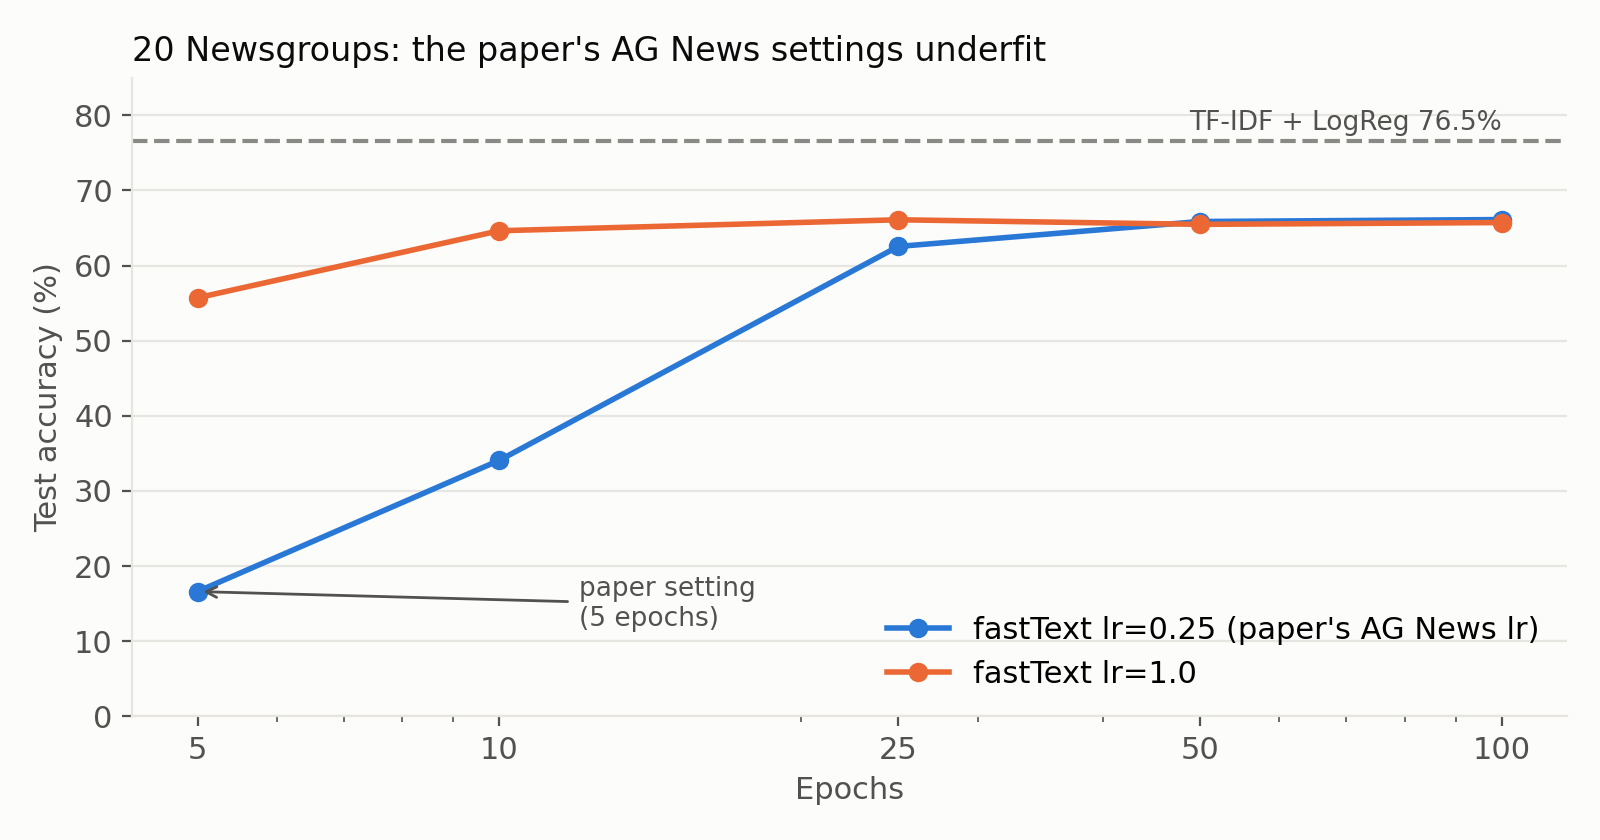
\includegraphics[width=\columnwidth]{20ng_epoch_sweep.png}
\caption{20 Newsgroups accuracy against training epochs (log scale), five seeds per point.
The paper's setting (5 epochs) badly underfits, and even the best setting stays below the
TF-IDF baseline.}
\label{fig:sweep}
\end{figure}

\subsection{2026 headlines: a twenty-year shift}
A model trained on AG News with the paper's settings reaches \XF\% $\pm$ \XFSD{} on the 2026
headlines, a drop of \XFdrop{} points from its in-domain \AGbi\%. Five-seed mean recall falls in every
class: World \XFrecWorld\%, Sports \XFrecSports\%, Business \XFrecBusiness\%, Sci/Tech
\XFrecSciTech\%. Business is hit hardest, with recall falling from \AGrecBusiness\% to
\XFrecBusiness\%. Figure~\ref{fig:cm} shows where accuracy is lost. The 2004 confusions
(Business~$\leftrightarrow$~Sci/Tech) are still there, and new leakage into World appears,
because many 2026 Business and Sci/Tech stories are about governments: EU membership, tax
pledges, oil prices during a war, and AI in elections. Vocabulary has shifted too. The NYT writes
``A.I.'', which the authors' tokenizer splits into \emph{a~.~i~.}, so the model never sees
the token \emph{ai}. Words such as \emph{openai} (13 items), \emph{chatgpt} and
\emph{deepfake} never occur in the AG News training data, so they are out of vocabulary.

Training fastText only on the 2026 data is much worse: \RSSin\% $\pm$ \RSSinSD{} from 407
training items, tested on the remaining 101. With the paper's settings and so few items,
fastText barely learns. TF-IDF logistic regression trained on the same 407 items reaches
\RSStf\%, close to the transfer result. For fastText, the old large corpus is far better than
a small new one, which matches the paper's framing of fastText as a method for large training
sets. A 101-item test set is too small for fine comparisons, so these in-domain numbers are
indicative only.

\begin{figure*}[t]
\centering
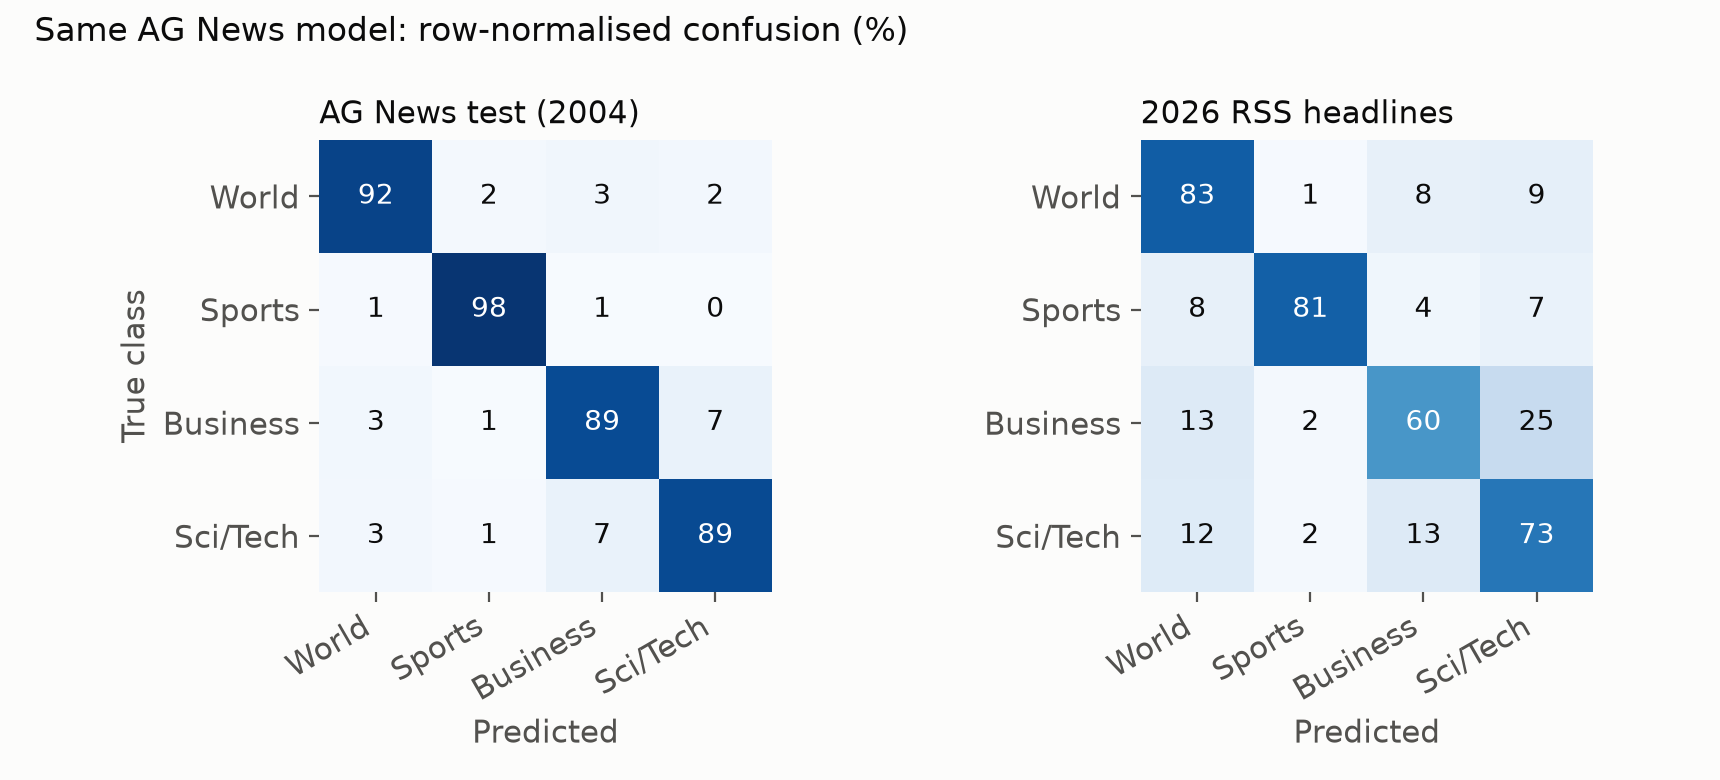
\includegraphics[width=0.78\textwidth]{confusion_agnews_vs_2026.png}
\caption{The same AG News-trained model (seed~0) on the AG News test set and on the 2026
headlines. Row-normalised; the diagonal is per-class recall. The recall figures in the text
are five-seed means, so they differ slightly from this single run.}
\label{fig:cm}
\end{figure*}

\subsection{LLM-as-judge: whose mistake is it?}
Accuracy treats every disagreement with the gold label as a model error. But the 2026 labels
come from newspaper sections, and the spot-check found them only 90\% clean. To separate
the causes, I used an LLM as a judge \citep{zheng2023judging} for every one of the \JudgeN{}
errors in one seed-0 run. The judge was Claude (\texttt{claude-opus-5-5}), given the
labelling guideline, the headline and lead sentence, the gold label and the predicted label,
but not the outlet. It answered with one verdict. \emph{MODEL\_ERROR} means the gold label
is clearly right. \emph{AMBIGUOUS} means both labels are defensible. \emph{LABEL\_NOISE}
means the gold label is wrong or no class fits. It also gave a one-line reason. The prompt
and all verdicts are in the repository.

The judge called \JudgeModel{} errors (\JudgeModelPct\%) genuine model errors, \JudgeAmb{}
(\JudgeAmbPct\%) ambiguous and \JudgeNoise{} (\JudgeNoisePct\%) label noise. For the judged run
(\XFseedZero\%), removing the items the judge called label noise raises accuracy to
\XFnoNoise\%. Also accepting the ambiguous cases raises it to \XFlenient\%. These figures depend
on the judge, so they are an estimate rather than a corrected accuracy. The genuine model
errors it found concentrate where the vocabulary changed: AI and technology stories
(\emph{A.I. agents}, OpenAI's mathematics results), and a video game review that a 2004 model
files under World because of the word \emph{war}.

\paragraph{Checking the judge.} I labelled a random 30 of the errors myself without seeing the
judge's verdicts. I worked from a separate sheet with only the headline, lead, gold and
predicted labels (in the repository), and the verdicts were merged in afterwards. We agreed on only \HumanAgree\% of them (Cohen's $\kappa$\,=\,\HumanKappa,
slight to fair agreement), and on \HumanBinary\% for the simpler question of whether the error
is the model's fault. The disagreements were systematic, not random. In 8 of the 16 cases the
judge called the gold label correct while I called it label noise. They included three economy
stories filed as Business (inflation, oil prices, household income) and several
science-section pieces with no clear Sci/Tech topic, such as a hurricane-centre profile. I was stricter than
the judge about what the feed sections mean. Both of us still put a large share of the errors
outside ``clear model error'': half of the 30 for the judge, and 20 of the 30 for me. So the
conclusion that the raw \XFdrop-point drop overstates the twenty-year shift holds under either
judgement. The exact split between noise, ambiguity and model error does not, because it
depends on who judges. The judge is therefore useful for sorting errors at scale, but not as a
replacement for a human annotator. Two humans and an adjudicated guideline would be the next
step.

\subsection{How the new results relate to the replication}
On data like AG News (short, balanced, four classes, large training set), the claim holds
exactly as published. Change the domain's length, number of classes or training size
(20~Newsgroups), and the paper's settings break. Tuning recovers part of the gap, and fastText
keeps its speed but not its parity with a stronger linear baseline. Change only the
\emph{time} (2026 headlines), and the architecture is unchanged but the learned vocabulary is
twenty years out of date. Both experiments evaluate differently from the replication: the
2026 test uses noisier, automatically derived labels, and the 20~Newsgroups setting had to be
tuned to be meaningful at all.

% ===================================================================
\section{Ethical Considerations}

\paragraph{The original paper.} \citet{joulin-etal-2017-bag} has no ethics statement, which
was normal before ACL venues introduced ethics review in 2021
\citep{benotti-blackburn-2022-ethics}. Looking back, using the benefits, harms and
vulnerable-groups framing of \citeauthor{benotti-blackburn-2022-ethics}:
(i)~\emph{Benefit}: efficiency is a real ethical gain. Training in seconds on a CPU instead of
hours on GPUs reduces energy use \citep{strubell-etal-2019-energy} and lets researchers
without large compute take part.
(ii)~\emph{Data}: five of its eight datasets (Yelp, Amazon, Yahoo!~Answers) are
user-generated text whose authors never agreed to become benchmarks and which can contain
personal details. AG News is scraped news distributed for non-commercial research. All are
mostly English and Western, so ``World'' means the world as seen from there.
(iii)~\emph{Dual use}: classification that is cheap at scale also makes automated content
filtering, censorship and surveillance cheap \citep{weidinger2021ethical}.

\paragraph{Publishing the new data.} Under the \emph{Australian Code for the Responsible
Conduct of Research} \citep{nhmrc2018code}, publishing this work raises the following issues.
Following \citet{karamolegkou-etal-2025-ethical}, I list actions taken, remaining concerns
and suggestions, rather than a disclaimer that there are none.

\emph{Respect and accountability: copyright.} The 2026 dataset contains headlines and lead
sentences owned by the BBC, The Guardian, NYT and ESPN, collected from public RSS feeds under
each outlet's terms. Copying them for research falls under fair dealing for research or
study (\emph{Copyright Act 1968}, s\,40). Redistributing them in a public repository is a
separate question. I keep the text, with the source link on every row, only to make the
results reproducible, and do not claim legal clearance. A version for wider publication
should release links, labels and the collection script only, and let users re-collect the
text, as is common for social-media datasets. I break that rule myself for now: the full text
is in the public repository so that the marker can reproduce every result. Once the unit is
marked, I will replace the text columns with links.

\emph{Respect: privacy.} The headlines name real people, including people involved in crime
and court stories. The text is already public, but collecting it freezes stories that the
publisher may later correct or remove. 20~Newsgroups contains real names and email addresses
from the 1990s. Removing headers and signatures was a privacy action as well as a fix for
label leakage.

\emph{Fairness.} All four outlets are UK or US, so the dataset encodes an Anglophone view of
what counts as world, business or science news. Arts and culture stories fit none of the four
classes and are forced into one or dropped. Source and class are partly confounded, so a
model may learn outlet style rather than topic. Adding non-Anglophone outlets and balancing
sources per class would reduce this.

\emph{Honesty, rigour and transparency.} I report the spot-check as single-annotator
agreement, not inter-annotator agreement. I report every seed and its spread, not the best
run. I keep the earlier Windows results next to the final ones. And I document the
LLM judge, its model and its prompt. Using an LLM judge sends dataset text to a third-party
service, and its output cannot be exactly reproduced, so the verdicts are stored rather than
regenerated. Generative AI (Claude) also helped with code and drafting. I checked all text,
numbers and references and am responsible for them.

\emph{Human research.} No human participants were involved. The only annotation was my own,
of public text, so under the \emph{National Statement on Ethical Conduct in Human Research}
\citep{nhmrc2023national} no human research ethics review was required.

% ===================================================================
\section{Conclusions and Reflections}

The replication worked. With the authors' code and settings, fastText reaches \AGbi\% on AG
News against a published 92.5\%, within seed-to-seed variation, and the speed advantage is
real. Generalisation is more mixed. The speed claim held everywhere I tested it, but the
accuracy claim did not. On 20~Newsgroups the published configuration underfits badly, and
even a tuned model trails a TF-IDF baseline by \NGbestGap{} points. On 2026 headlines a model
trained on 2004 news loses \XFdrop{} points, part of which is label noise in my own data
rather than model failure. ``About as accurate'' turns out to depend on short texts, few
classes, plenty of training data and a stable vocabulary.

Three things would change if I started again. First, I would collect the 2026 data over
several weeks from the start rather than on one day, since a single news cycle is a thin
sample. Second, I would build the labels from a guideline-driven annotation instead of
feed sections. Feeds are cheap, but the 40 cross-filed stories and the LLM-judge results
show how much of the measured error they cause. Third, I would record every run's seed,
thread count and platform from the first day. Rerunning everything in one batch at the end
was the only way to get a consistent results file.

\section*{Limitations}
Replication covers AG News only, not all eight datasets of the original paper, and the
best 20~Newsgroups setting was chosen on the test set. The 2026
dataset is small (508 usable items), comes from one day and four Anglophone outlets, and
its labels come from feed sections checked on a 50-item sample by one person. The LLM judge
is a single model in a single pass, and it agreed only weakly with my own judgements
($\kappa$\,=\,\HumanKappa). The UCI dataset from the proposal was not run.

\bibliography{custom}

\end{document}
